\documentclass[tikz,border=4pt]{standalone}
% Estilo común de los diagramas de bloques (se usa con \input en cada standalone)
\usepackage[defaultsans,scale=0.92]{lato}
\usepackage{libertinust1math}
\usepackage{xcolor,amsmath}
\usepackage{tikz}
\usetikzlibrary{positioning,arrows.meta,calc,shapes.geometric}
\usepackage{../../notacion}
\definecolor{ctrlazul}{HTML}{1E5AA8}\definecolor{ctrlnoche}{HTML}{14213D}
\definecolor{ctrlcoral}{HTML}{D1495B}\definecolor{ctrlverde}{HTML}{2A9D8F}
\definecolor{ctrlambar}{HTML}{E09F3E}\definecolor{ctrlgris}{HTML}{5C677D}
\definecolor{ctrlvioleta}{HTML}{6C4AB6}\definecolor{ctrlteal}{HTML}{0F7173}
\tikzset{
  >={Stealth[length=2.4mm]}, every node/.style={font=\small},
  bloque/.style={draw=ctrlnoche,fill=ctrlazul!7,thick,rounded corners=1.5pt,minimum height=9mm,minimum width=13mm,inner sep=4pt},
  suma/.style={draw=ctrlnoche,thick,circle,inner sep=0pt,minimum size=6mm},
  senal/.style={->,thick,draw=ctrlnoche},
  rot/.style={font=\footnotesize,text=ctrlgris},
}

\begin{document}
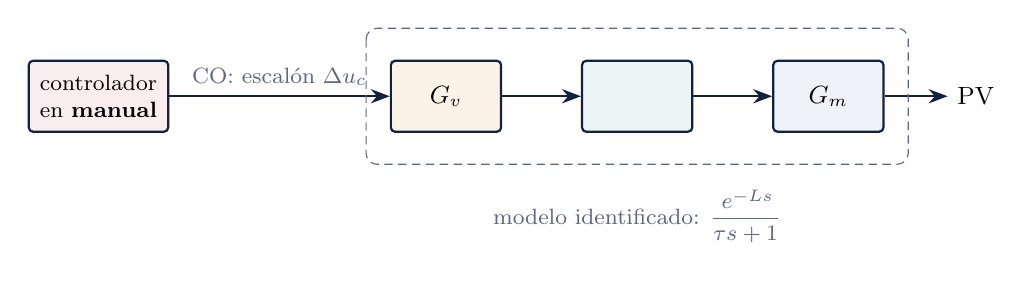
\begin{tikzpicture}[b/.style={bloque,minimum width=14mm}]
  \node[b,fill=ctrlcoral!10,align=center,font=\footnotesize] (c) {controlador\\en \textbf{manual}};
  \node[b,right=28mm of c,fill=ctrlambar!12] (v) {$G_v$};
  \node[b,right=10mm of v,fill=ctrlverde!10] (p) {$\Gp$};
  \node[b,right=10mm of p] (m) {$G_m$};
  \node[right=8mm of m] (y) {PV};
  \draw[senal] (c)--node[above,rot]{CO: escalón $\Delta u_c$}(v);
  \draw[senal] (v)--(p); \draw[senal] (p)--(m); \draw[senal] (m)--(y);
  \draw[densely dashed,ctrlgris,rounded corners] ($(v.north west)+(-3mm,4mm)$) rectangle ($(m.south east)+(3mm,-4mm)$);
  \node[rot,below=6mm of p] {modelo identificado: $\dfrac{\Kproc\,e^{-Ls}}{\tau s+1}$};
\end{tikzpicture}
\end{document}
